\documentclass[conference]{IEEEtran}
\IEEEoverridecommandlockouts
% The preceding line is only needed to identify funding in the first footnote. If that is unneeded, please comment it out.
\usepackage{cite}
\usepackage{amsmath,amssymb,amsfonts}
\usepackage{algorithmic}
\usepackage{graphicx}
\usepackage{textcomp}
\usepackage{xcolor}
\usepackage{tikz}
\usepackage{adjustbox}
\usetikzlibrary{positioning}
\def\BibTeX{{\rm B\kern-.05em{\sc i\kern-.025em b}\kern-.08em
    T\kern-.1667em\lower.7ex\hbox{E}\kern-.125emX}}

\begin{document}

\title{Guitar Percussive Classification for Control of an External System\\
}

\author{\IEEEauthorblockN{Oliver Whorwood}
\IEEEauthorblockA{\textit{School of Electronic Engineering and Computer Science} \\
\textit{Queen Mary University of London}\\
London, UK \\
ec21904@qmul.ac.uk}
}

\maketitle

\begin{abstract}
This paper outlines the design and development of a guitar percussive classification system for parameter control of effects. The need for such a system stems from a proposed
requirement in conjunction with HyVibe who manufacture a guitar amplification system which uses actuators placed onto the inside of a guitar body. Currently, the way to control these parameters is either
through the use of physical buttons or a separate wireless guitar pedal.
The system proposed uses a CNN based approach to achieve around 75\% accuracy for a realistic scenario involving triggering a parameter change whilst simultaneously playing a series of chords and performing some percussive guitar.
A full, end-to-end system is built which successfully predicts an incoming signal in real-time and uses this to change an effect on the HyVibe system.

\end{abstract}
 
\section{Introduction}
The direction of solving this problem will be through the use of some form of spectral processing and will not require interaction with any hardware apart from the guitar itself.

A piezoelectric sensor underneath the saddle of a guitar produces a small electrical signal which is amplified to line level by the HyVibe system, this will then be used to determine
any interaction occurring on the guitar.

Several onset detection techniques will be researched, specifically relating to percussive onsets as this most closely relates to the task at hand.

A real-time classification system will need to be built to recognise control taps and send a MIDI message to the controller to change certain parameters.

The system will be evaluated using objective measures such as F-measure for the offline system, overall latency for the real-time system and subjective ease of use of the whole system.

The aim is to have a system that can detect two types of control taps to send out two different control messages when the user is playing normal plucked or strummed guitar simultaneously.

\section{Literature review}
In a review of current onset detection techniques in the scope of Automatic Drum Transcription (ADT), it is noted that this task is more challenging than with pitched instruments
due to the wide frequency response produced and onsets which tend to be noisy (Wu et al., 2018). It groups current techniques into several methods: ``Segmentation-Based'', ``Classification-Based'', ``Language-Based''
and ``Activation-Based''. ``Segmentation-Based'' methods tend to use simple Onset Detection Functions based around the envelope of the signal. This has the advantage of being very simple
to implement however this method tends to perform poorly when other types of instrument, particularly pitched, are added to the mix. ``Classification-Based'' methods are based around
a more complex input representation combining things such as spectral centroid, RMS energy and Mel-Frequency Cepstral Coefficients. The input representation can be finely tuned to increase
the accuracy of classification. This still suffers from interference of melodic instruments if these have not been introduced in the training phase.``Language-Based'' methods use language
models such as Hidden Markov Models (HMMs) to detect patterns in the features of the audio. It is not commonly used in ADT scenarios as the structure of music does not follow patterns
as closely as natural language. Modern ``Activation-Based'' methods use either Non-negative Matrix Factorisation (NMF) or Recurrent Neural Network (RNN) and produce easy to interpret
outputs and can also be used in source separation tasks. They can suffer from degradation due to sources overlapping. This section also outlines the use of CNNs in the most recent papers. 
The paper concludes that the RNN based approaches tend to be the most accurate. CRNN and CNN methods are not evaluated. 

Earlier methods related specifically to guitar onset detection use spectral methods (Mounir, Karsmakers and van Waterschoot, 2016). Specifically this paper compares, the then 'state of the art' method of spectral flux, to a novel method of looking at the sparsity of the magnitude spectrogram.
This shows an improved F-measure for the new method up to 1.000 for normal guitar notes. There is mention of filtering of the audio to remove, but it is not specific about the type or amount of filtering applied. 

A paper for Automatic Drum Transaction found three different methods worked better in different contexts (Southall, Stables and Hockman, 2017). These are a Soft Attention Bidirectional RNN (SA), BRNN with Peripheral Connections (PC) and a CNN.
The SA involves using an RNN with weighted connections allowing weights to be brought to the output from previous time steps through hidden layers. The PC method follows a similar setup but has
direct connections from previous time steps to the output. To increase the input feature size without requiring extensive computation time, a CNN system is also proposed. The evaluation uses a dataset which includes acoustically
separated drum sounds, combined drum sounds and those with other instruments included. The accuracy is determined via an F-measure. 
It was found that the SA method performed better for cases where the context was known i.e. just percussion or a mix of percussion and polyphonic. The CNN performed better in the 
scenarios where the context was unknown. The context of this paper's proposed system is unknown as the \emph{control taps} could take place alongside other pitched sounds from the strings
therefore a CNN based approach will be considered. 

A CNN neural network aims to detect spacially invariant patterns (O'Shea and Nash, 2015). A filter consisting of weights is shifted along the input one element at a time (with a stride of 1) and with each iteration the result is summed.
The translation invariance means that the pattern can be shifted to different positions in the input and still be detected. Ultimately, the dense layer will determine how different locations of matches
are weighted. Supervised learning will take place which involves using inputs that are labelled beforehand and the model learns the patterns which relate to each label.

Classification of other types of percussive sound is explored by (Rohit, Bhattacharjee and Rao, 2021). It aims to classify hits to the Northern Indian originating tabla instrument, consisting of two hand-struck drums. This will likely be more similar to the
type of harmonic content produced from percussive guitar. One of their approaches uses a CNN model which consists of two convolution and max pooling layers followed by two dense layers with dropout, this one-way model
is tuned for each of the four stroke types and outperforms the more complex three-way model however a separate model for each class would require an increase in computational time. The dataset contained a huge number of hits with 26,600 in the training set and a further 4,470 in the test set. 

An efficient CNN based approach for onset detection has been proposed (Schluter and Bock, 2014) which uses two convolutional filters followed by a fully connected layer. This method is used to detect
downbeat positions in a range of genres of music and outperforms other competing methods such as RNN and SuperFlux. The F-measure of the CNN system is 0.885 compared to 0.873 for RNN. The reproducibility of 
this proposed architecture could be improved by providing open source code, however it is described is much detail. This
is shown to be improved upon further by adding dropout, something which needs to be considered here, especially with a small dataset which can suffer from overfitting (Srivastava et al., 2014). The dropout layer
removes weights from random neurons to perform regularisation to the network.

There are many sections of a guitar which can be struck to produce a sound, these can be split into harmonic and inharmonic components, the strings produce mainly harmonic content when
struck whereas the body of the guitar produces mainly inharmonic content (Itoyama et al., 2007). The harmonicity refers to the relationship of frequencies where there are integer multiples of the fundamental frequency.
Many guitar players also use the inharmonic components to act as percussion. 

The \emph{control tap} locations are designed to be as ergonomic as possible, particularly considering existing research on injury due to guitar playing (Marmaras and Zarboutis, 1997). Three experienced guitarists are observed and interviewed regarding their playing
style and fatigue as a result. The study suggests that for the control parts of the guitar in particular, these should not cause wrist flexion or extensions. 

There has been research undertaken regarding the location and types of percussive guitar gestures (Martelloni, McPherson and Barthet, 2020). Several interviews took place to determine the most likely hand positions used for percussion. These
are collated and summarised in a diagram as can be seen in Fig \ref{percussion-areas}. This is a very good starting point for deciding which areas to include in a novel dataset as well as being very specific on the hand positions used in each one.
The participants consisted of four men and one women, so the range of percussive styles explored may not represent the wider guitar playing community especially in other cultures. 

\begin{figure}[htbp]
    \centerline{\includegraphics[scale=0.4]{percussion-areas.png}}
    \caption{Location of common percussion areas (Martelloni, McPherson and Barthet, 2020)}
    \label{percussion-areas}
    \end{figure}

Datasets have been produced previously on percussive onsets occurring on different parts of a guitar as part of a design of an augmented guitar to produce percussive sounds (Martelloni, McPherson and Barthet, 2021). However, the method of recording these percussive taps is through piezoelectric sensors placed at various locations not
including an under-saddle position. As the proposed \emph{control taps} would be from areas not used for percussive guitar, it would be difficult to combine this dataset with new recordings.

There is however, a dataset that contains guitar playing through a hexaphonic pickup for use as an augmented dataset (Xi et al., 2018). This covers a wide range of genres, musical styles recorded by six professional musicians.
This wide range of different notes, chords and picking/strumming patterns provides a good example of the context that the onsets would be presented in. The hexaphonic pickup is a magnetic coil type which is clipped onto the guitar which picks
up vibration in the strings themselves by causing a change in the magnetic flux. This is in comparison to the piezoelectic sensor the physical vibrations in the saddle of the guitar where the compressions in the sensor produce an electrical signal (Lemme, 2009).

The latency of the system needs to be low enough to not have a detrimental effect on playability. For musicians even a delay of 20ms is noticeable (Jack et al., 2018). This value is determined through a series of experiments involving both musicians
and non-musicians including subjective quality, perception and accuracy. Jitter, the change in the absolute latency was found to also have a profound impact, where even a latency of 10ms is noticeable if it is not stable over time. This paper however
focusses on musical percussive performance latency whereas the system proposed will be used for control of effects, so the tolerance may well be higher.

The parts of the guitar that are focussed on are the front body, divided into the lower and upper bout, the bridge, and the side (Bay, 2013). The positions of these can be seen in Fig. \ref{guitar}.

\begin{figure}[htbp]
    \centerline{\includegraphics[scale=0.4]{guitar.png}}
    \caption{Labelled parts of an acoustic guitar. (Bay, 2013)}
    \label{guitar}
    \end{figure}


Experimental acoustic analysis has shown that guitar bodies with visual symmetry also display acoustic symmetry in that plane and that the internal brace structure of the guitar has a profound impact on the nodes pattern produced on the soundboard (Mihălcică, Stanciu and Vlase, 2020).
Adding more bars to the braces increased the amount of overtones (other harmonics). 

The means of real-time communication is determined by the protocol type used by the HyVibe system. It has the provision of MIDI over Bluetooth Low Energy (BLE) to control certain parameters (HyVibe SA, 2022). The real-time system will
make use of libraries built for this purpose, however the overall architecture must be understood. In a BLE `connection', the `central' device scans for packets on the network from devices which could be connected and 
is responsible for starting the connection (Tosi et al., 2017). The `peripheral' accepts connections. In this scenario the HyVibe system is the `central' device and controls all the settings. The made benefit of this protocol is
its low energy capability, with a power consumption approximately 1.5 times lower than the similar protocol `ANT+'. 


\section{Methodology}
The system will make use of the HyVibe System Installation Kit which consists of an under-saddle piezoelectric pickup, main controller unit, a connection panel for audio and charging, and two actuators (HyVibe SA, 2021).
This system is installed on an existing electroacoustic guitar, which will be referred to as the ``Tanglewood'', with its piezoelectric sensor replaced. The main controller unit and connection panel are not installed due to incompatibility with the existing slots in
the body of the guitar. Instead, the cable for the piezoelectric sensor is fed through a slot in the body to be connected to the rest of the electronics which remain outside the guitar. This experimental setup can be
seen in Fig. \ref{tanglewood-setup}. External sounds are less likely to be picked up than with a microphone, so the dataset collection is not undertaken in anechoic conditions, but the guitar is rested on a soft surface to reduce any low
vibrations reaching the sensor.

\begin{figure}[htbp]
    \centerline{\includegraphics[scale=0.4]{tanglewood-setup.png}}
    \caption{The Tanglewood guitar setup with the HyVibe system plugged in. The approximate location of the internal brace is shown in blue.}
    \label{tanglewood-setup}
    \end{figure}

The first experiment is to test the performance of a CNN model to detect one type of onset and tune the hyperparameters accordingly. There will be one \emph{control tap} used to trigger a parameter change on the HyVibe system. Based on the percussive guitar research, it is decided to have the \emph{control tap} as a single-finger tap on the bridge area, to the side of
the saddle, the location of which is detailed in Fig. \ref{tanglewood-taps}. This will be known as \emph{bridge tap}. The \textbf{initial} dataset is created which involved stopping any movement of the guitar strings by baffling them with a cloth. One hundred \emph{bridge taps} are recorded and hand annotated, these are varied as much as possible
in terms of the tap velocity and the exact location of impact on the bridge, each tap uses either the first or second finger. The dataset is shuffled to have a random selection of 80\% for training with a remaining 20\% reserved for offline testing. 

\begin{figure}[htbp]
    \centerline{\includegraphics[scale=0.4]{tanglewood-taps.png}}
    \caption{Location of the control/bridge tap (green), lower-bout tap (purple) and side slap (yellow)}
    \label{tanglewood-taps}
    \end{figure}

To quantify the accuracy of the model, the F-measure is calculated using the true positives, false positives and false negatives produced from the prediction. This is calculated automatically using the equation \[\dfrac{tp}{tp+\dfrac{1}{2}(fp+fn)}\] (Taha and Hanbury, 2015).

As seen in Fig. \ref{system}, the analogue signal output from the piezoelectric sensor is amplified by the HyVibe system before being converted to a digital signal using an external audio interface. The audio interface used is an Audient iD4 using the front D.I. with a gain setting of 5. The datasets are recording into a Digital Audio Workstation (DAW), Logic Pro, along to
a metronome set at a rate of 60bpm. The audio files are recorded at a sample rate of 44.1kHz, 24-bit dynamic range in WAVE uncompressed format. The onsets occur at approximately one second intervals however these intervals are not accurate. Therefore, these files are imported 
to another DAW, Audacity, where the onsets are labelled manually and exported as a text file with each onset's absolute time position in seconds. This text file has two columns relating to the onset start and end time but, as this is annotated as being instantaneous, only the first column is used.

\begin{figure}[htbp]
    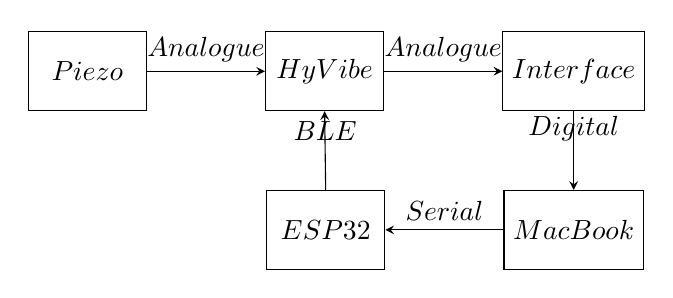
\begin{tikzpicture}
     
    \node[draw,
        minimum height=1cm,
        minimum width=1.5cm,
        fill=white]
        (piezo) at (0,0){$Piezo$};
    
    \node[draw,
        minimum height=1cm,
        minimum width=1.5cm,
        right=1.5cm of piezo,
        fill=white]
        (hyvibe) {$HyVibe$};
    
    \node[draw,
        minimum height=1cm,
        minimum width=1.5cm,
        right=1.5cm of hyvibe,
        fill=white]
        (interface) {$Interface$};
    
    \node[draw,
        minimum height=1cm,
        minimum width=1.5cm,
        below=1cm of interface,
        fill=white]
        (macbook) {$MacBook$};
    
    \node[draw,
        minimum height=1cm,
        minimum width=1.5cm,
        left=1.5cm of macbook,
        fill=white]
        (esp) {$ESP32$};
    
    \draw[-stealth] (piezo.east) -- (hyvibe.west)
        node[midway,above]{$Analogue$};
    
    \draw[-stealth] (hyvibe.east) -- (interface.west)
        node[midway,above]{$Analogue$};
    
    \draw[-stealth] (interface.south) -- (macbook.north)
        node[midway,above]{$Digital$};
    
    \draw[-stealth] (macbook.west) -- (esp.east)
        node[midway,above]{$Serial$};
    
    \draw[-stealth] (esp.north) -- (hyvibe.south)
        node[midway,above]{$BLE$};
     
    \end{tikzpicture}
    \caption{An overview of the system architecture.}
    \label{system}
    \end{figure}

It is important that the control taps are not too audible when compared to normal guitar playing as this could distract from a performance, the average amplitude of these compared to normal guitar playing will be calculated.

A script is developed to train a neural network model and evaluate its performance, this is written is Python using the TensorFlow library. This, along with the datasets can be found at https://github.com/whorwood/MastersProject. To train the detection system, the audio signal is first converted to the frequency domain via a Short-Time Fourier Transform (STFT) using the `librosa' Python library. The output is windowed
using 15 time-bin wide sections shifting by 1 each time with a corresponding ground truth relating to the presence of an onset at the centre of the window.

The neural network itself is based around the structure of (Schluter and Bock, 2014). The model is started with the structure: convolution (3x7) with 10 features, maxpool (3x1), convolution (3x3) with 20 features, maxpool (3x1), flatten, Dense (256), Dense (1).
The hyperparameters of the neural network are refined by testing their performance in a tap onset detection task. First, the hop size of the FFT is decreased to 1024 from 2048 improving the F-measure from 0.9895 to 0.9967. This is decreased again by half to check this trend,
however a hop size of 512 reduces the F-measure down to 0.980 so a hop size of 1024 is fixed. Next, the size of the filters are increased to see their effect on accuracy. The hypothesis is that this will increase the accuracy as the filter size will then be
more proportional to the input size. The filters are set to sizes of (12,7) and (12,3). With all other parameters unchanged, this in fact decreases the detection accuracy to an F-measure of 0.9931 disproving the hypothesis. The network depth is also reduced to a single layer to assess the impact
and as expected this also decreases the overall accuracy to 0.9861. Not by a huge margin, however the initial structure must be as refined as possible. This simplification of the network will of course reduce computational time so is considered for the real-time system. 
Finally, the number of neurons is the final dense layer is both decreased to 128 and increased to 512, both with the effect of decreasing overall accuracy.

The model and weights from each training session are saved for future evaluation. The model itself is saved in JSON, a human-readable data format designed to be lightweight and cross-compatible (Nurseitov et al., 2009) and the weights are contained within the Keras specific H5 format. 

Two non-control onsets are now introduced, a single-finger tap on the lower-bout area and a slap-like gesture using the underside of the hand on the side of the guitar body, both of which are illustrated again in Fig. \ref{tanglewood-taps}. These are two common areas where percussive guitar would occur, thus
it is important to see if a system could detect the differences between each type of onset location. This dataset now consists of one hundred \emph{bridge taps}, one hundred \emph{lower-bout taps} and one hundred \emph{side slaps}. Again, the strings are baffled in all scenarios hence the dataset name \textbf{Muted\_String}.
The ground truth is now an array of 3 integers, corresponding to an occurrence of each type of onset. The output of the model is modified to a multi-label sigmoid function, so the final layer becomes: Dense (3). 

Next, the \textbf{Muted\_String} dataset is replicated but without the strings being muted, so they are free to resonate as they would in normal guitar playing, this is called \textbf{Open\_String}. No fingerboard fingering occurs during this dataset, so the resonance of the strings is related 
to the most commonly used open tuning (Sparks, 1997): E (82.41 Hz), A (110.00 Hz), D (146.83 Hz), G (196.00 Hz), B (246.94 Hz), E (329.63 Hz) (Suits, 2022). The model is then evaluated on this new dataset by training and testing.

A more realistic scenario for the \emph{control taps} to occur is whilst or directly after the strings have been strummed or picked with various fingerings on the fretboard. To test the model's performance on this in a controlled manner, an \textbf{Augmented} dataset is created. 
This is done by overlaying the \textbf{Open\_String} dataset with sections from the ``GuitarSet'' dataset. The ``GuitarSet'' dataset uses a hexaphonic pickup which records each string individually. These six tracks are summed together
to create a single output like that of a normal mono-output pickup. The gain of the audio being overlaid is adjusted to be at the same relative amplitude as the onsets. This is achieved by recording a similar style of playing on the acoustic guitar and measuring the amplitude, then adjusting
the gain of the ``GuitarSet'' audio to match this amplitude. Excepts from the five musical styles in the dataset from the first player are overlaid onto each track. 

As it is now established how well the model can perform at detecting each separate type of onset, the model is simplified into a binary classifier either detecting a \emph{control tap} or anything else (guitar playing, \emph{lower-bout taps} or \emph{side slaps}). 
This is first evaluated on the \textbf{Open\_String} dataset, then this dataset is appended by a further one hundred \emph{control taps} to ensure that when performing the binary classification the dataset is balanced between the two classes. This is called \textbf{Open\_String\_Balanced}. 
These additional \emph{control taps} are overlaid with the same \textbf{GuitarSet} excerpts as before, creating an \textbf{Augmented\_Balanced} dataset to be compared with the multi-label classification.

The dataset is still fairly limited with four hundred total onsets, to increase the diversity of the dataset a further two hundred \emph{control taps}, one hundred \emph{lower-bout taps} and one hundred \emph{side slaps} are recorded and annotated. As before these are augmented, creating an \textbf{Augmented\_Extended} dataset. 

Another guitar, manufactured by \emph{LAG} and with a HyVibe system installed is used to create a new dataset following exactly the same procedure as \textbf{Open\_String\_Balanced}.

To test the feasibility of a real-time classification system, a prototype is developed to recognise the onsets of three positions of tapping in real-time and send one MIDI message to the HyVibe system.
The real-time detection system is written in Python and sends serial messages to an ESP32 development board which is programmed in C++ to send a MIDI message whenever a serial
message of `1' is received. If a threshold of 0.5 is reached for a control tap prediction, and the previous prediction was 0, then the serial message is sent.
This then triggers the MIDI message of type `note-off' to be sent to the HyVibe system over BLE, on channel 1 and note number 1. On the HyVibe system this is configured to trigger the ``Loop record met'' function
which activates the looper recording proceeded by a metronome count in (HyVibe SA, 2022).

A special dataset is created to test the taps along/away from the internal brace structure which involved placing tape as close as possible along the location of the brace and creating a recording of one hundred taps along this brace and another one hundred not along the 
brace. These two datasets are named \textbf{Along\_Brace} and \textbf{Away\_Brace} respectively. 

The final stage of onset detection testing involves using the \emph{LAG} guitar as an end-user would with a combination of typical guitar playing, percussive taps and \emph{control taps}. 
To maximize reproducibility potential, a defined set of chords are played along with specific tapping locations. The order of playing is as follows: G Major, D Major, A Minor, \emph{bridge tap}, G Major, D Major, A Minor, \emph{lower-bout tap}, G Major, D Major, A Minor, \emph{side slap} with a one second interval between each event.
This entire sequence is repeated twenty-five times with the guitar strummed using a plectrum and another twenty-five times strummed using the first finger.

To check that the real-time system is performing as expected in an automated manner, pre-recorded audio from a dataset that the model being used is trained on is looped back into the audio interface to simulate real-time playback on the guitar. With each onset detected, two successive MIDI messages are broadcast, a `note-on'
followed by a `note-off' which are recorded in the DAW using a `virtual instrument' track. The MIDI status bytes for these messages are 0x90 and 0x80 (Ellinger, 2014). These message locations are then checked against the onsets in the recording being played to calculate an F-measure.


\section{Results \& Discussion}
The best accuracy for the hyperparameter selection in the initial tests was found to be 0.9934 by using a (3x7) and (3x3) filter size, FFT size of 1024 and dense layer of 256 neurons.
At a sample rate of 44.1kHz, this relates to an actual window width of 93ms, which is already established as being ideal for music related tasks (McFee et al., 2015). 

The first evaluation involves the \textbf{Muted\_String} dataset. This was run for ten epochs with a batch size of 32, with the epochs being established based on the number required for the loss to reach the `knee' point. 
The F-measure for each class is 0.9770, 0.9691 and 0.9711 with an average of 0.9724.
There are more false positives than false negatives for the \emph{control tap} and \emph{lower-bout tap} but the opposite for \emph{side slap} suggesting that there are more similar frequency and spatial characteristic
between the \emph{control taps} and \emph{lower-bout taps} with \emph{side slaps} having a more unique response. This intuitively makes sense as the location of the \emph{side slap} is on a completely different face of
the guitar as well as using the back of the hand rather than a finger tap. 

In terms of the amplitude of the onsets, these on average sit around the -32dB point for the open string \emph{control taps}. There will be a huge range of amplitude for all sorts of guitar playing, but a test of playing chords 
with a plectrum had a range of approximately -24dB to -22dB. This at most represents a 10-fold higher SPL for the guitar playing than the onsets which is more than enough to be almost completely perceptually masked.

\begin{figure}[htbp]
    \centerline{\includegraphics[scale=0.4]{classif-open.png}}
    \caption{Loss function over time for the multi-label classification of the \textbf{Open\_String} dataset}
    \label{classif-open}
    \end{figure}

For the \textbf{Open\_String} dataset, after thirty epochs the F-measures are 0.9877, 0.9797 and 0.9691, with an average of 0.9788. The loss function for this training can be seen in Fig. \ref{classif-open}. The initial assumption was that this would decrease the accuracy
due to the added frequencies from the resonating strings however there is actually a slight increase. When looking at the spectrogram of the guitar onsets containing string sounds compared to the muted strings,
the main structure of the onset is fairly low in frequency, so the resonance does not interact enough for differentiation of the onsets to be obscured. 

For the \textbf{Augmented} dataset, after thirty epochs the F-measures are 0.9211, 0.8220 and 0.8959, an average of 0.8797. This augmentation causes a slight decrease in accuracy as now the signal overlaying the onsets
is higher in amplitude than the freely resonating strings. The same pattern of accuracy across the different onsets can be seen, where the \emph{bridge taps} have a higher accuracy than the other two onset types. This could be
explained by the higher average signal level of the \emph{bridge taps} which are around 2dB higher than the other onsets, producing more defined patterns in the spectrogram.

Next, for the binary classification model, the \textbf{Open\_String} dataset in this scenario achieves an F-measure of 0.9782, and with \textbf{Open\_String\_Balanced}: 0.9901. The performance remains similar to the multi-label classfication for the unbalanced
dataset which suggests that actually all three onset types can be differentiated well otherwise the model would see a bigger increase in performance when the two percussive types are combined to one label. Having a balanced dataset increases
the accuracy as previously there was probably bias towards the other onset types.

The equivalent test on \textbf{LAG} with open strings has an F-measure of 0.9855 after thirty epochs. This is lower than the ``Tanglewood'' accuracy even with the gain matched for the onsets which occur in the same equivalent locations on both guitars. The subtle difference in the
harmonic response could be less favourable in terms of pattern recognition.

\textbf{Augmented\_Balanced} has an F-measure of 0.9406. As expected, this is less accurate as there are now instances of other frequency content overlapping the control taps making them harder
to distinguish. A good example of this can be seen in Fig. \ref{augmented-bridge} at an instance where the onset is completely masked by a chord being played on the guitar. This is still a good accuracy considering how similar the onsets of the guitar chords
look to the \emph{bridge taps}.

\begin{figure}[htbp]
    \centerline{\includegraphics[scale=0.4]{augmented-bridge.png}}
    \caption{The SFTF of an onset occurring in the augmented dataset}
    \label{augmented-bridge}
    \end{figure}


\textbf{Augmented\_Extended} has an F-measure of 0.9383. It can be seen here that in this instance, the larger dataset decreased accuracy by a very small margin, not what is expected. The increase in variation in the
dataset could be the cause, and this model would likely perform better when used with a completely unknown, new dataset compared to the non-extended model.
With a random dropout of 20\% added between the two dense layers, the F-measure remains very similar with a slight decrease at 0.9317.

\textbf{LAG\_Augmented} achieves a good F-measure of 0.8955, slightly lower than the equivalent test on the ``Tanglewood''. This is the same pattern seen for the non-augmented dataset, where the ``Tanglewood'' again performs better.

The real-time script has to complete each prediction step in time for the next audio buffer. Currently, that script is being executed on a 2.9 GHz Quad-Core Intel Core i7 based system. Initially, each audio buffer was incrementing
by a single STFT time bin each iteration which did not allow sufficient time for the predictions to take place. The other extreme considered was to increment by the full network input width of fifteen bins, however if the onset extends
across the boundary of two windows, there might not be enough information for a correct prediction. When looking at the spectrogram output, it was noticed that the majority of the frequency content of the onset is contained within three 
consecutive bins. Therefore, a compromise was made of iterating twelve bins so that there is always an overlap of three.

The real-time system is also tested for latency in three scenarios, first when triggered by an onset tap, then from a keyboard press from Python, and finally a button press directly from the
ESP32 board. These scenarios will determine where the sources of latency occur. The latency for the fist scenario is measured by recording the audio output from the guitar and measuring the time difference between the first audio peak in the onset and the first audio peak in the metronome.
The second scenario is measured by sending a MIDI message internally to the DAW on a key press (enter) which is recorded alongside the audio output. For the third scenario the button is pressed at the same time as a note on a MIDI keyboard, which is recorded in the DAW. 
Each scenario is tested five times and the average latency is calculated. For the onset trigger, the total latency is a fairly substantial 1167.4ms. Comparing this with sending
the serial message directly from the Python script via a keyboard press, the latency is 1037.4ms. Finally, when the button is used, the latency is less than 1ms.
There is a serious bottleneck in the system at the serial communication layer. The onset detection itself only accounts for an average of 130ms of latency. Other methods to relay the signal
from Python may have to be considered.

\begin{figure}[htbp]
    \centerline{\includegraphics[scale=0.04]{LAG-setup.jpg}}
    \caption{The experimental setup for the LAG guitar}
    \label{acoustic-bridge}
    \end{figure}

With an initial subjective test of the real-time system, it seemed that percussive taps occurring at positions over the internal braces were more likely to be misclassified as control taps, hypothesised that due to the acoustic resonance here being more similar to the bridge which is also structurally attached to
the braces. The is evaluated further by creating two new datasets of percussive taps, one with taps occurring above the internal braces and one with taps occurring away from the internal braces. The F-measure is then calculated for each of these datasets.
Figure shows the approximate location of these braces in the guitar under test, this will vary with different guitars, but a similar principal can be applied. This hypothesis is disproven as the F-measure for the dataset over the brace is actually slightly higher than the 
one away from the brace at 0.9709 compared to 0.9518. It could be that the proximity of the tap to the bridge has more of an effect than whether it occurs over a brace, this would need to be verified by further experimentation. 

When using the weights trained on the \textbf{Open\_String\_Balanced} dataset and using this to predict control onsets on the LAG guitar, this performed poorly with an F-measure of 0.240. This can be improved slightly be decreasing the classification threshold from 0.5 to 0.1 reaching
a maximum F-measure of 0.264. This shows that the harmonic resonance produced by taps to the equivalent locations on different guitars vary significantly and that the generalisation of the model is low. The reverse of this process is also tested, so using the LAG trained model to predict
onsets in the \textbf{Open\_String\_Balanced} dataset. The F-measure was slightly higher at 0.4547 and did not increase with lower threshold values. When observing the spectrogram representation of an example of a \emph{control tap} on the \emph{Tanglewood} guitar compared to the \emph{LAG},
it can be seen that the frequency response varies a lot between the two, shown in Fig. \ref{acoustic-bridge} and Fig. \ref{LAG-bridge}.

\begin{figure}[htbp]
    \centerline{\includegraphics[scale=0.4]{acoustic-bridge.png}}
    \caption{The STFT frequency response of an open string onset on the ``Tanglewood'' guitar}
    \label{acoustic-bridge}
    \end{figure}

\begin{figure}[htbp]
    \centerline{\includegraphics[scale=0.4]{LAG-bridge.png}}
    \caption{The STFT frequency response of an open string onset on the ``LAG'' guitar}
    \label{LAG-bridge}
    \end{figure}
    
The models trained on the augmented datasets are also tested in the same manner. For the \textbf{LAG\_Augmented} trained model, tested on the \textbf{Augmented\_Balanced} (``Tanglewood'') dataset, this achieved a maximum F-measure of 0.4471 at a threshold of 0.1. For the other way round, the F-measure was even lower at 0.3300 at the same threshold of 0.1. This is similar to what is seen with the open string datasets
and further suggests that the frequency characteristics vary a lot between the two guitars.

Both these tests show that the models trained on a single guitar type are too overfit when used to predict onsets on another guitar. To try to combat this, the model is trained on a combination of datasets from both guitars. Before, the training/test split is undertaken after the shuffling of the dataset,
however now the datasets for both guitars must be kept separate for evaluation, so the shuffling occurs after the training/test split. The combined model is tested against the test set from both the Open\_String as well as the LAG and the performance improved significantly achieving 
an F-measure of 0.9852 and 0.9832 respectively.

The weights trained on the augmented dataset are evaluated further by using the \textbf{LAG\_playing} dataset, a realistic scenario involving a mixture of guitar playing and different taps. This again performed quite poorly with an F-measure of 0.4170 at a threshold of 0.1. This was slightly surprising as the onsets themselves
were produced in the same way as the open string dataset. The guitar playing sections are slightly higher amplitude than the average for the augmented audio causing different masking of the onsets which is probably throwing the model off.

The model is then trained using the \textbf{LAG\_playing} dataset, which is the most likely continuing steps for implementing a releasable version of the system. For this to be realised fully, the dataset would have to be expanded across many different guitars and players, and playing techniques. When using this single dataset
from one player on one guitar, an F-measure of 0.752 is achieved. The dataset would ideally be expanded to including a playing scenario on the \emph{tanglewood} guitar however this could not be achieved due to the HyVibe system not being installed securely in this guitar meaning it has to remain on a flat
surface during dataset collection.

The real-time system evaluation had an F-measure of 1, as there was perfect detection of all onsets. This is expected as the real-time system uses the same model implementation with the only difference being the method and libraries used
for reading in the real-time audio stream. 

Subjectively, using the system to control effects was quite temperamental in terms of the accuracy and false triggers which impeded the natural flow of guitar playing. Once the script is executed, this keeps running without any faults or errors and the predictions reliably complete on time.

\section{Conclusions \& Further Work}

A CNN based approach developed for detecting downbeats in music transfers well to the task of detecting percussive onsets from a hollow bodied acoustic guitar, a dataset related to a real world scenario achieved an F-measure of 0.7520.

The latency of the overall prototype system is high which for controlling some parameters such as starting and stopping loops will be much more noticeable than turning on and off effects such as reverb. This latency however is due to a serial interface between two devices which would be 
negated in a system with inbuilt BLE capability. The system works as expected as a whole with a complete solution from the control tap, through the real-time detection system which successfully changes parameters on the HyVibe system.

There is insignificant difference in performance when taps are positioned around internal structures in the guitar, in this case the brace connected to the bridge.

Changing guitar has a large effect on the accuracy of trained models and don't generalise well. By using a combined dataset for training, this improved the performance when using this model to predict for both guitars. 

In this case a dropout layer did not improve the accuracy of the augmented extended model, different degrees of dropout and other layer combinations could be evaluated in further studies. 

The realistic playing dataset would need to be expanded significantly to create one that was representative of a variety of guitar players and styles. With the datasets and models provided open source, this has the potential to be expanded by further studies.

The \emph{control tap} is not noticeable when combined with `normal' guitar playing due to the large difference in amplitude. The system was able to successfully detect taps that have minimal force.

To determine which locations and techniques for control taps would be the most suitable for guitar players, a user study would have to take place. The original aim of having two control taps is not met, however as it is determined
that the system can successfully differentiate between different onset types, it is likely that a second control tap would be able to be introduced.

\begin{thebibliography}{00}

\bibitem{} Wu, C., Dittmar, C., Southall, C., Vogl, R., Widmer, G., Hockman, J., Muller, M. and Lerch, A. (2018) ``A Review of Automatic Drum Transcription'', IEEE/ACM Transactions on Audio, Speech, and Language Processing, 26(9), pp. 1457-1483. doi: 10.1109/taslp.2018.2830113.    
\bibitem{} Mounir, M., Karsmakers, P. and van Waterschoot, T. (2016) "Guitar note onset detection based on a spectral sparsity measure", 2016 24th European Signal Processing Conference (EUSIPCO). doi: 10.1109/eusipco.2016.7760394.
\bibitem{} Southall, C., Stables, R. and Hockman, J. (2017) ``Automatic Drum Transcription for Polyphonic Recordings Using Soft Attention Mechanisms and Convolutional Neural Networks'', ISMIR.
\bibitem{} O'Shea, K. and Nash, R. (2015) ``An introduction to convolutional neural networks.'', ArXiv, abs/1511.08458.
\bibitem{} Rohit, A., Bhattacharjee, A. and Rao, P. (2021) ``FOUR-WAY CLASSIFICATION OF TABLA STROKES WITH MODELS ADAPTED FROM AUTOMATIC DRUM TRANSCRIPTION'', ISMIR.
\bibitem{} Schluter, J. and Bock, S. (2014) ``Improved musical onset detection with Convolutional Neural Networks'', 2014 IEEE International Conference on Acoustics, Speech and Signal Processing (ICASSP). doi: 10.1109/icassp.2014.6854953.
\bibitem{} Srivastava, N., Hinton, G., Krizhevsky, A., Sutskever, I. and Salakhutdinov, R. (2014) ``Dropout: a simple way to prevent neural networks from overfitting'', Journal of Machine Learning Research, 15(1), pp. 1929–1958.
\bibitem{} Itoyama, K., Goto, M., Komatani, K., Ogata, T. and Okuno, H. (2007) "Integration and Adaptation of Harmonic and Inharmonic Models for Separating Polyphonic Musical Signals", 2007 IEEE International Conference on Acoustics, Speech and Signal Processing - ICASSP '07. doi: 10.1109/icassp.2007.366615.
\bibitem{} Marmaras, N. and Zarboutis, N. (1997) ``Ergonomic redesign of the electric guitar'', Applied Ergonomics, 28(1), pp. 59-67. doi: 10.1016/s0003-6870(96)00032-4.
\bibitem{} Martelloni, A., McPherson, A. and Barthet, M. (2020) "Percussive Fingerstyle Guitar through the Lens of NIME: an Interview Study", New Interfaces for Musical Expression (NIME).
\bibitem{} Martelloni, A., McPherson, A. and Barthet, M. (2021) "Guitar augmentation for Percussive Fingerstyle: Combining self-reflexive practice and user-centred design", Proceedings of the International Conference on New Interfaces for Musical Expression.
\bibitem{} Xi, Q., Bittner, R., Pauwels, J., Ye, X. and Bello, J. (2018) "Guitarset: A Dataset for Guitar Transcription", in 19th International Society for Music Information Retrieval Conference. Paris, France.
\bibitem{} Jack, R., Mehrabi, A., Stockman, T. and McPherson, A. (2018) ``Action-sound Latency and the Perceived Quality of Digital Musical Instruments'', Music Perception, 36(1), pp. 109-128. doi: 10.1525/mp.2018.36.1.109.
\bibitem{} Bay, C. (2013) Glossary of guitar terms. Pacific, MO: Mel Bay.
\bibitem Mihălcică, M., Stanciu, M. and Vlase, S. (2020) "Frequency Response Evaluation of Guitar Bodies with Different Bracing Systems", Symmetry, 12(5), p. 795. doi: 10.3390/sym12050795.
\bibitem{} HyVibe SA (2022) MIDI Instructions. Available at: https://www.hyvibeguitar.com/airturn-midi-instructions/ (Accessed: 12 August 2022).
\bibitem{} Tosi, J., Taffoni, F., Santacatterina, M., Sannino, R. and Formica, D. (2017) ``Performance Evaluation of Bluetooth Low Energy: A Systematic Review'', Sensors, 17(12), p. 2898. doi: 10.3390/s17122898.
\bibitem{} HyVibe SA (2021) HyVibe System Installation Instructions. Available at: https://www.hyvibeguitar.com/wp-content/uploads/2021/05/HyVibe-Installation-Instructions-EN.pdf (Accessed: 12 August 2022).
\bibitem{} Ellinger, J. (2014) MIDI Basics. Available at: https://people.carleton.edu/~jellinge/m208w14/pdf/02MIDIBasics\_doc.pdf (Accessed: 12 August 2022).
\bibitem{} Nurseitov, N., Paulson, M., Reynolds, R. and Izurieta, C. (2009) ``Comparison of JSON and XML Data Interchange Formats: A Case Study'', Caine, 9, pp. 157-162.
\bibitem{} Sparks, P. (1997) ``Guitar Performance in the Nineteenth Centuries and Twentieth Centuries'', Performance Practice Review, 10(1), pp. 71-79. doi: 10.5642/perfpr.199710.01.07.
\bibitem{} Suits, B. (2022) Frequencies of Musical Notes, A4 = 440 Hz, Physics of Music Notes. Available at: https://pages.mtu.edu/~suits/notefreqs.html (Accessed: 12 August 2022).
\bibitem{} McFee, B., Raffel, C., Liang, D., Ellis, D., McVicar, M., Battenberg, E. and Nieto, O. (2015) "librosa: Audio and music signal analysis in python", Proceedings of the 14th python in science conference, 8, pp. 18-25. 
\bibitem{} Lemme, H. (2009) BuildYourGuitar.com :: The Secrets of Electric Guitar Pickups. Available at: https://a.pomf.cat/zjnuis.pdf (Accessed: 13 August 2022).
\bibitem{} Taha, A. and Hanbury, A. (2015) "Metrics for evaluating 3D medical image segmentation: analysis, selection, and tool", BMC Medical Imaging, 15(1). doi: 10.1186/s12880-015-0068-x.

\end{thebibliography}
\vspace{12pt}

\section{Appendix}
\begin{table}[!ht]
     \centering
     \begin{adjustbox}{width=\textwidth}
     \begin{tabular}{|l|l|l|l|l|l|l|l|l|l|l|l|l|l|l|}
        \hline
        Number & Trained on & Dense Outputs & Filter Size & FFT Size & Classification type & Dataset & Epochs & Label & TP & FP & FN & F-measure & Final Loss & Notes \\ \hline
        1 & ~ & 256 & 3,7,3,3 & 2048 & Binary & Initial & 10 & ~ & 282 & 4 & 2 & 0.989473684 & 0.0133 & ~ \\ \hline
        2 & ~ & 256 & 3,7,3,3 & 1024 & Binary & Initial & 10 & ~ & 301 & 1 & 1 & 0.996688742 & 0.0066 & ~ \\ \hline
        3 & ~ & 256 & 3,7,3,3 & 512 & Binary & Initial & 10 & ~ & 270 & 3 & 12 & 0.972972973 & 0.0037 & ~ \\ \hline
        4 & ~ & 256 & 12,7,12,3 & 1024 & Binary & Initial & 10 & ~ & 284 & 0 & 5 & 0.991273997 & 0.0065 & ~ \\ \hline
        5 & ~ & 256 & 3,3 & 1024 & Binary & Initial & 10 & ~ & 320 & 5 & 4 & 0.986132512 & 0.0061 & ~ \\ \hline
        6 & ~ & 512 & 3,7,3,3 & 1024 & Binary & Initial & 10 & ~ & 324 & 6 & 0 & 0.990825688 & 0.0065 & ~ \\ \hline
        7 & ~ & 128 & 3,7,3,3 & 1024 & Binary & Initial & 10 & ~ & 324 & 8 & 0 & 0.987804878 & 0.0072 & ~ \\ \hline
        8 & ~ & 256 & 3,7,3,3 & 1024 & Multilabel & Muted\_String & 10 & 0 & 297 & 14 & 0 & 0.976973684 & 0.0031 & ~ \\ \hline
        8 & ~ & 256 & 3,7,3,3 & 1024 & Multilabel & Muted\_String & 10 & 1 & 282 & 14 & 4 & 0.969072165 & 0.0031 & ~ \\ \hline
        8 & ~ & 256 & 3,7,3,3 & 1024 & Multilabel & Muted\_String & 10 & 2 & 286 & 5 & 12 & 0.971137521 & 0.0031 & ~ \\ \hline
        9 & ~ & 256 & 3,7,3,3 & 1024 & Multilabel & Open\_String & 10 & 0 & 295 & 11 & 3 & 0.976821192 & 0.003 & ~ \\ \hline
        9 & ~ & 256 & 3,7,3,3 & 1024 & Multilabel & Open\_String & 10 & 1 & 274 & 6 & 9 & 0.973357016 & 0.003 & ~ \\ \hline
        9 & ~ & 256 & 3,7,3,3 & 1024 & Multilabel & Open\_String & 10 & 2 & 281 & 4 & 3 & 0.987697715 & 0.003 & ~ \\ \hline
        10 & ~ & 256 & 3,7,3,3 & 1024 & Multilabel & Open\_String & 30 & 0 & 320 & 2 & 6 & 0.987654321 & 0.0004 & ~ \\ \hline
        10 & ~ & 256 & 3,7,3,3 & 1024 & Multilabel & Open\_String & 30 & 1 & 314 & 8 & 5 & 0.979719189 & 0.0004 & ~ \\ \hline
        10 & ~ & 256 & 3,7,3,3 & 1024 & Multilabel & Open\_String & 30 & 2 & 298 & 15 & 4 & 0.969105691 & 0.0004 & ~ \\ \hline
        11 & ~ & 256 & 3,7,3,3 & 1024 & Multilabel & Augmented & 30 & 0 & 257 & 18 & 26 & 0.921146953 & 0.005 & ~ \\ \hline
        11 & ~ & 256 & 3,7,3,3 & 1024 & Multilabel & Augmented & 30 & 1 & 224 & 36 & 61 & 0.822018349 & 0.005 & ~ \\ \hline
        11 & ~ & 256 & 3,7,3,3 & 1024 & Multilabel & Augmented & 30 & 2 & 241 & 14 & 42 & 0.895910781 & 0.005 & ~ \\ \hline
        12 & ~ & 256 & 3,7,3,3 & 1024 & Binary & Augmented\_Extended & 30 & ~ & 1110 & 50 & 96 & 0.938292477 & 0.0085 & ~ \\ \hline
        13 & ~ & 256 & 3,7,3,3 & 1024 & Binary & Open\_String & 30 & ~ & 292 & 10 & 3 & 0.978224456 & 0.0011 & ~ \\ \hline
        14 & ~ & 256 & 3,7,3,3 & 1024 & Binary & Open\_String\_Balanced & 30 & ~ & 602 & 6 & 6 & 0.990131579 & 0.0021 & ~ \\ \hline
        15 & ~ & 256 & 3,7,3,3 & 1024 & Binary & Augmented\_Balanced & 30 & ~ & 562 & 42 & 29 & 0.940585774 & 0.0054 & ~ \\ \hline
        16 & 14 & 256 & 3,7,3,3 & 1024 & Binary & Along\_Brace & 0 & ~ & 17203 & 283 & 0 & 0.991841794 & ~ & ~ \\ \hline
        17 & 15 & 256 & 3,7,3,3 & 1024 & Binary & Along\_Brace & 0 & ~ & 16497 & 989 & 0 & 0.970897213 & ~ & ~ \\ \hline
        18 & 14 & 256 & 3,7,3,3 & 1024 & Binary & Away\_Brace & 0 & ~ & 17140 & 231 & 0 & 0.993306482 & ~ & ~ \\ \hline
        19 & 15 & 256 & 3,7,3,3 & 1024 & Binary & Away\_Brace & 0 & ~ & 15775 & 1596 & 0 & 0.951849394 & ~ & ~ \\ \hline
        20 & 15 & 256 & 3,7,3,3 & 1024 & Binary & LAG & 0 & ~ & 589 & 1294 & 2434 & 0.240114146 & ~ & Thresh - 0.5 \\ \hline
        20 & 15 & 256 & 3,7,3,3 & 1024 & Binary & LAG & 0 & ~ & 644 & 1483 & 2379 & 0.250097087 & ~ & Thresh - 0.3 \\ \hline
        20 & 15 & 256 & 3,7,3,3 & 1024 & Binary & LAG & 0 & ~ & 691 & 1587 & 2332 & 0.260705527 & ~ & Thresh - 0.2 \\ \hline
        20 & 15 & 256 & 3,7,3,3 & 1024 & Binary & LAG & 0 & ~ & 731 & 1788 & 2292 & 0.263803681 & ~ & Thresh - 0.1 \\ \hline
        21 & ~ & 256 & 3,7,3,3 & 1024 & Binary & LAG & 30 & ~ & 578 & 10 & 7 & 0.985507246 & 0.0019 & ~ \\ \hline
        22 & ~ & 256 & 3,7,3,3 & 1024 & Binary & LAG\_Augmented & 30 & ~ & 523 & 28 & 94 & 0.895547945 & 0.0063 & ~ \\ \hline
        23 & 23 & 256 & 3,7,3,3 & 1024 & Binary & LAG\_Playing & 0 & ~ & 145 & 10 & 605 & 0.320441989 & ~ & Thresh - 0.5 \\ \hline
        23 & 23 & 256 & 3,7,3,3 & 1024 & Binary & LAG\_Playing & 0 & ~ & 171 & 15 & 579 & 0.365384615 & ~ & Thresh - 0.3 \\ \hline
        23 & 23 & 256 & 3,7,3,4 & 1024 & Binary & LAG\_Playing & 0 & ~ & 182 & 19 & 568 & 0.382754995 & ~ & Thresh - 0.2 \\ \hline
        23 & 23 & 256 & 3,7,3,5 & 1024 & Binary & LAG\_Playing & 0 & ~ & 206 & 32 & 544 & 0.417004049 & ~ & Thresh - 0.1 \\ \hline
        24 & ~ & 256 & 3,7,3,6 & 1024 & Binary & LAG\_Playing & 30 & ~ & 123 & 54 & 27 & 0.752293578 & 0.0011 & ~ \\ \hline
        25 & 22 & 256 & 3,7,3,7 & 1024 & Binary & Open\_String\_Balanced & 0 & ~ & 1682 & 2702 & 1333 & 0.454656035 & ~ & Thresh - 0.5 \\ \hline
        25 & 22 & 256 & 3,7,3,8 & 1024 & Binary & Open\_String\_Balanced & 0 & ~ & 1749 & 2996 & 1266 & 0.450773196 & ~ & Thresh - 0.3 \\ \hline
        26 & 16 & 256 & 3,7,3,9 & 1024 & Binary & LAG\_Augmented & 0 & ~ & 450 & 138 & 2573 & 0.249238438 & ~ & Thresh - 0.5 \\ \hline
        26 & 16 & 256 & 3,7,3,10 & 1024 & Binary & LAG\_Augmented & 0 & ~ & 522 & 208 & 2501 & 0.278177458 & ~ & Thresh - 0.3 \\ \hline
        26 & 16 & 256 & 3,7,3,11 & 1024 & Binary & LAG\_Augmented & 0 & ~ & 583 & 272 & 2440 & 0.300670449 & ~ & Thresh - 0.2 \\ \hline
        26 & 16 & 256 & 3,7,3,12 & 1024 & Binary & LAG\_Augmented & 0 & ~ & 673 & 383 & 2350 & 0.329982839 & ~ & Thresh - 0.1 \\ \hline
        27 & 23 & 256 & 3,7,3,13 & 1024 & Binary & Augmented\_Balanced & 0 & ~ & 1243 & 1422 & 1772 & 0.437676056 & ~ & Thresh - 0.5 \\ \hline
        27 & 23 & 256 & 3,7,3,14 & 1024 & Binary & Augmented\_Balanced & 0 & ~ & 1351 & 1715 & 1664 & 0.444334813 & ~ & Thresh - 0.3 \\ \hline
        27 & 23 & 256 & 3,7,3,15 & 1024 & Binary & Augmented\_Balanced & 0 & ~ & 1417 & 1918 & 1598 & 0.446299213 & ~ & Thresh - 0.2 \\ \hline
        27 & 23 & 256 & 3,7,3,16 & 1024 & Binary & Augmented\_Balanced & 0 & ~ & 1543 & 2345 & 1472 & 0.447052006 & ~ & Thresh - 0.1 \\ \hline
        28 & ~ & 256 & 3,7,3,17 & 1024 & Binary & Open\_String\_Balanced+LAG & 30 & ~ & ~ & ~ & ~ & ~ & 0.0019 & ~ \\ \hline
        29 & 29 & 256 & 3,7,3,18 & 1024 & Binary & Open\_String\_Balanced & 0 & ~ & 566 & 11 & 9 & 0.982638889 & ~ & ~ \\ \hline
        30 & 29 & 256 & 3,7,3,19 & 1024 & Binary & LAG & 0 & ~ & 592 & 11 & 8 & 0.984206151 & ~ & ~ \\ \hline
        31 & ~ & 256 & 3,7,3,20 & 1024 & Binary & Augmented\_Extended & 30 & ~ & 1146 & 108 & 60 & 0.931707317 & 0.0104 & Dropout - 0.2 \\ \hline
        
     \end{tabular}
 \end{adjustbox}
 \end{table}

\end{document}